\documentclass{book}
\usepackage{ctex}
\usepackage{xcolor}
\usepackage{hyperref}
\usepackage{graphics}

\title{\Large Git tutorial }

\author{LeeMoo}


\begin{document}

\maketitle
\tableofcontents
\subsection{}
The entire pro Git book, written by Scott Chacon and Ben Straub and published by Apress, is availble here. All conteent is licensed under the Creative Commons Attribution Non Commericial Share Alike 3.0 license. Print versions of the book are available on \href{www.amazon.com}{Amazon.com}.\\

\chapter{起步}
	\section{关于版本控制}
	\subsection{关于版本控制}
	\paragraph{}
	什么是版本控制?我为什么要关心它呢?版本控制是一种记录一个或若干个文件内容变化,以便将来查阅特定版本修订情况的系统。在配中所展示的例子中,我们仅对保存着软件源代码的广西文件作版本控制管理,但实际上,你可以对任何类型的文件进行版本控制。\\
	如果你是位图形或网页设计师,可能会需要保存某一幅图片或页面布局文件的所有修订版本(这或许是你非常渴望拥有的功能)。采用版本控制系统(VCS)是个明智的选择。有了它你就可以将某个文件回溯到之前的状态,你可以比较文件的变化细节,查出最后是谁修改了哪个地方,从而找出导致怪异问题的原因,又是谁在何时报告了某个功能缺陷等等.使用版本控制系统通常是意味着,就算你乱来一气把整个项目的文件改的改删的删,你也照样可以轻松恢复到原先的样子.但额外增加的工作量却微乎其微。\\
	\subsection{本地版本控制系统}
	\paragraph{}
许多人习惯用复制整个项目目录的方式来保存不同的版本,或许还会改名加上备份的时间以示区别.这么做唯一的好处就是简单.不过坏处也不少:有时候会混淆所在的工作目录,一旦弄错文件丢了数据就没法撤销恢复.\\
	为了解决这个问题,人们很久以前就开发了许多种本地版本控制系统,大多都是采用某种简单的数据库来记录文件的历次更新差异(如图1-1)。\\
	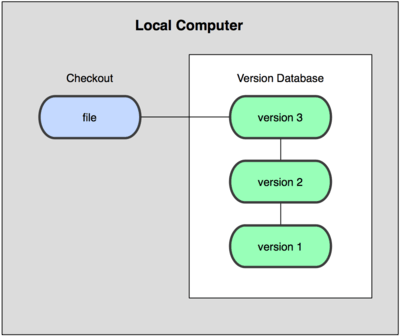
\includegraphics{1-1.png}\\
	\其中最流行的一种叫做RCS,现今许多计算机系统上都还看得到它的踪影.甚至在流行的Mac OSX 系统上安装了开发者工具包之后,也可以使用RCS命令.它的工作原理基本上就是保存并管理文件补丁(patch)。文件补丁是一种特定格式的广西文件,记录着对应文件修订前后的内容变化。所以,根据每次修订后的补丁,RCS可以通过不断打补丁,计算出各个版本的文件内容。\\
	\subsection{集中化的版本控制系统}
	\paragraph{}
	接下来人们又遇到一个问题,如何让在不同系统上的开发者协同工作?于是,集中化的版本控制系统(CVCS)应运而生.这类系统,诸如CVS,Subversion以及Perforce等,都有一个单一的集中管理的服务器,保存所有文件的修订版本,而协同工作的人们都通过客户端连到这台服务器,取出最新的文件或者提交更新.多年以来,这已成为版本控制系统的标准做法(见图1-2)\\
	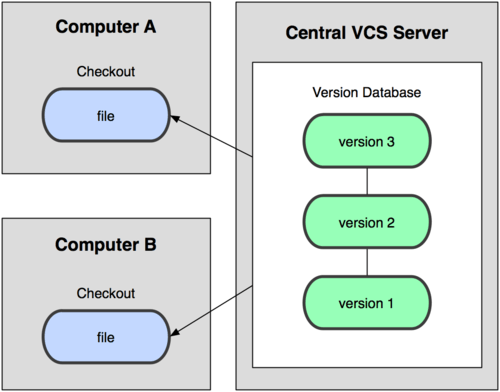
\includegraphics{1-2.png}\\
	这种做法带来了许多好处,特别是相较于老式的本地VCS来说。现在每个人都可以在一定程序上看到项目中的其他人正在做些什么.而管理员也可以轻松掌控每个开发者的权限,并且管理一个CVCS要远比在各个客户端维护本地数据库来得轻松容易。\\
	事分两面,有好有坏。这么做最显而易见的缺点是中央服务器的单点故障。如果宕机一小时,那么在这一小时内,谁都无法提交更新,也就无法协同工作.要是中央服务器的磁盘发生故障,碰巧没做备份,或者备份不够及时,就会有丢失数据的风险.最坏的情况是彻底丢失整个项目的所有历史更改记录,而被客户端偶然提取出来的保存在本地的某些快照数据就成了恢复数据的希望.但这样的话依然是个问题,你不能保证所有的数据都已经有人事先完整提取出来过.本地版本控制系统也存在类似问题,只要整个项目的历史记录被保存在单一位置,就有丢失所有历史更新记录的风险.\\
	\subsection{分布式版本控制系统}
	\paragraph{}
	于是分布式版本控制系统(DVCS)面世了。在这类系统中,像Git,Mercurial,Bazaar 以及Darcs等,客户端并不只提取最新版本的文件快照,而是把代码仓库完整地镜像下来.这么一来,任何一处协同工作用的服务器发生故障,事后都可以用任何一个镜像出来的本地仓库恢复。因为每一次的提取操作,实际上都是对代码仓库的完整备份(见图1-3)。\\
	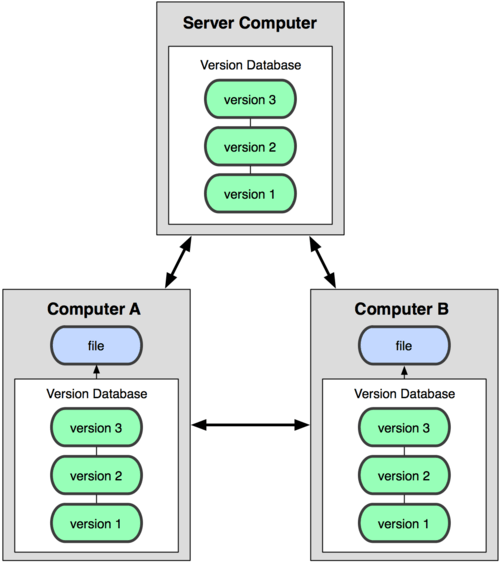
\includegraphics{1-3.png}\\
	更进一步,许多这类系统都可以指定和若干不同的远端代码仓库相互协作.你可以根据需要设定不同的协作流程,比如层次模型式的工作流,而这在以前集中式系统中是无法实现的.\\

	\section{Git简史}
	\subsection{Git简史}
	同生活中的许多伟大事件一样,Git诞生于一个极富纷争大举创新的年代。Linux内核开源项目有着为数众多的参与者.绝大多数的Linux内核维护工作都花在了提交补丁和保存归档的繁事务上(1991--2002年间)。到2002年,整个项目组开始雇用分布式控制系统BitKeeper来管理和维护代码。\\
	到了2005年,开发BitKeeper的商业公司同Linux内核开源社区的合作关系结束,他们收回了免费使用BitKeeper的权力。这就迫使Linux开源社区(特别是Linux的缔造者Linus Torvalds)不得不吸取教训,只有开发一套属于自己的版本控制系统才不至于重蹈覆辙。他们对新的系统制订了目标:\\
	\begin{itemize}
		\item 速度
		\item 简单的设计 
		\item 对非线性开发模式的强力支持(允许上千个并行开发的分支)
		\item 完全分布式
		\item 有能力高效管理类似Linux内核一样的超大规模项目(速度和数据量)
	\end{itemize}\\
	\paragraph{}
	自诞生于2005年以来,Git日臻成熟完善,在高度易用的同时,仍然保留着初期设定的目标。它的速度飞快,极其适合管理大项目,它还有着令人难以置信的非线性分支管理系统(见第三章),可以就会各种复杂项目开发需求。\\
	\section{Git基础}
	\subsection{Git 基础}
	\paragraph{}
	那么,简单地说,Git空间是怎样的一个系统呢?请注意,接下来的内容非常重要,若是理解了Git的思想和基本工作原理,用起来就会知其所以然,游刃有余.在开始学习git的时候,请不要尝试把各种概念和其他版本控制系统相比拟,否则容易混淆每个操作的实际意义。Git在保存和处理各种信息的时候,虽然操作起来的命令形式非常相近,但它与其他版本控制系统的做法颇为不同.理解这些差异将有助于你准确地使用Git提供的各种工具。\\
	\subsection{直接记录快照,而非差异比较}
	\paragraph{}
	Git和其他版本控制的主要差别在于,Git只关心文件数据的整体是束发生变化,而大多数其他系统则只关心文件内容的具体差异。这类系统每次记录有哪些文件作了更新,以及都更新了哪些行的什么内容,请看图1-4。\\
	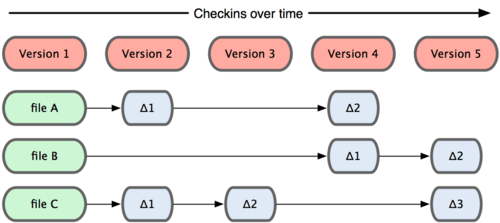
\includegraphics{1-4.png}\\
	Git并不保存这些前后变化的差异数据.实际上,Git更像是把变化的文件作快照后, 记录在一个微型的文件系统中.每次提交更新时,它会纵览一遍所有文件的指纹信息并对文件作一快照,然后保存一个指向这个快照的索引。为提高性能,若文件没有变化,Git不会再次保存,而只对上次保存的快照作一链接。Git的工作方式就像图1-5所示。\\
	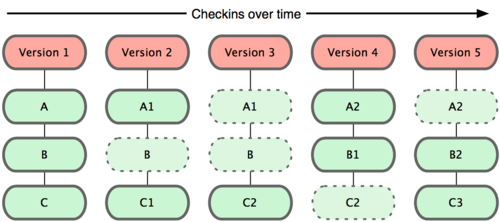
\includegraphics{1-5.png}\\
	这是Git同其他系统的重要区别.它完全颠覆了传统版本控制的套路,并对各个环节的实现方式作了新的设计。Git更像一个小弄的文件系统,但它同时还提供了许多以此为基础的超强的工具,而不只是一个简单的VCS。稍后在第三章讨论Git分支管理的时候,我们会再看看这样的设计空间会带来哪些好处。\\

	\subsection{近乎所有操作都是本地执行}
	在Git中的绝大多操作都只需要访问本地文件和资源,不用联网。但如果用CVCS的话,差不多所有操作都需要连接网络。因为Git在本地磁盘上就保存着所有当前项目的历史更新,所以处理起来速度飞快。\\
	举个例子,如果要浏览项目的历史更新摘要,Git不用跑到外面的用品上去取数据回来,而直接从本地数据库读取后展示给你看。所以任何时候你都可以马上翻阅,无需等待。如果想要看当前版本的文件和一个月之前的版本之间有何差异,Git会取出一个月前的快照和当前文件作一次差异运算,而不用请求远程来做这件事,或是把老版本的文件拉到本地来作比较。\\
	用CVCS的话,没有网络或者断开VPN你就无法做任何事情,但用Git的话,就算你在飞机或者火车上,都可以非常愉快地频繁提交更新,等到了有网络的时候再上传到远程仓库。同样,在回家的路上,不用连接VPN你也可以继续工作。换作其他版本控制系统,这么做几乎不可能,抑或非常麻烦。看上去这都不是什么大问题,但实际体验后,你会惊喜地发现,这其实会带来很大不同的。\\
	\subsection{时刻保持数据完整性}
	\paragraph{}
	在保存到git之前,所有数据都要进行内容的校验和计算(checksum),并将此结果作为数据的唯一标识和索引。换句话说,不可能在你修改了文件或目录之后,Git一无所知。这项特性作为Git的设计哲学,建在整体架构的最底层。所以如果文件在传输时变得不完整,或者磁盘损坏导致文件数据缺失,Git都能立即察觉。\\
	Git使用SHA-1算法计算数据的校验和,通过对文件的内容或目录的结构计算出一个SHA-1哈唏值,作为指纹字符串,该字符串由40个十六进制字符(0-9及a-f)组成,看起来就像:\\
	\begin{minipage}[c]{0.8\textwidth}
		\fbox{
			\bf 24b9da6552252987aa493b52f8696cd6d3b00373
		}
	\end{minipage}\\
	Git的工作完全信赖于这类指纹字串,所以你会经常看到这样的啥希值。实际上所有保存在Git数据库中的东西都是用此啥希值来作索引的,而不是靠文件名。\\
	\subsection{多数操作仅添加数据}
	常用的Git操作大多仅仅是把数据添加到数据库。因为任何一种不可逆的操作,比如删除数据,都会使回退或重现历史版本变得困难重重。在别的VCS中,若还未提交更新,就有可能丢失或者混淆一些修改的内容,但在Git里,一旦白净净快照之后,就完全不用担心丢失数据,特别是养成定期摄像头到其他仓库的习惯的话。\\
	这种高可靠性令我们的开发工作安心不少,尽管去做各种试验性的尝试好了,再怎样也不会弄丢数据。至于Git内部究竟是如何保存和恢复数据的,我们会在第九章订座Git内部原理时再作详述。\\
	\subsection{文件的三种状态}
	\paragraph{}
	好,现在请注意,接下来要讲的概念非常重要。对于任何一个文件,在Git内都只有三种状态:已提交(committed),已修改(modified)和已暂存(staged)。已提交表示该文件已经安全地保存在本地数据库中了;已修改表示了某个文件,但还没有提交保存;已暂存表示把已修改的文件放在下次提交时要保存的清单中。\\
	由此我们看到Git管理项目时,文件流转的三个工作区域:Git的工作目录,暂存区域,以及本地仓库。\\
	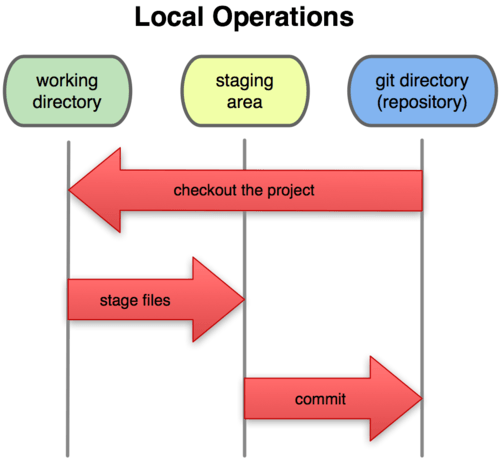
\includegraphics{1-6.png}\\
	每个项目都有一个Git目录(注释:如果\textcolor{red}{\textbf{git clone}}出来的话,就是其中\textcolor{red}{\textbf{.git}}的目录;如果\textcolor{red}{\textbf{gti clone -\,-bare}}的话,新建的目录本身就是Git目录。),它是Git用来保存元数据和对象数据库的地方。该目录非常重要,每次克隆镜像仓库的时候,实际拷贝的就是这个目录里面的数据。\\
	从项目中取出某个版本的所有文件和目录,用以开始后续工作的叫做工作目录。这些文件实际上都是从Git目录中的压缩对象数据库中提取出来的,接下来就可以在工作目录是中对这些文件进行编辑。\\
	所谓的暂存区域只不过是个简单的文件,一般都放在Git目录中。有时候人们会把这个文件叫做索引文件,不过标准说法还是叫暂存区域。\\
	基本的Git工作流程如下:\\
	\begin{enumerate}
		\item 在工作目录中修改某些文件。\\
		\item 对修改后的文件进行快照,然后保存到暂存区域。\\
		\item 提交更新,将保存在暂存区域的文件快照永久转储到Git目录中。\\
	\end{enumerate}
	所以,我们可以从文件所处的位置来判断状态:如果是Git目录中保存着的特定版本文件,就属于已提交状态;如果作了修改已放入暂存区域,就属于已暂存状态;如果自上次取出后,作了修改但还没有放到暂存区域,就是已修改状态。到第二章的时候,我们会进一步了解其中细节,并学会如何根据文件状态实施后续操作,以及怎样跳过暂存直接提交。\\
	\section{安装Git}
	\subsection{安装Git}
		一般的Linux都会自带Git。如果你用的是Windows的话,算了,你还是用VS2013社区版的吧!\\
	
	\section{初次运行Git前的配置}
	一般在新的系统上,我们都需要先配置下自己的Git工作环境。配置工作只需要一次,以后升级时还会沿用现在的配置。当然,如果需要,你随时可以用相同的命令修改已有的配置。\\
	Git提供了一个叫做\textbf{git config}的工具(译注:实际是\textbf{git-config}命令,只不过可以通过加一个名字来呼叫此命令。),专门用来配置或读取相应的工作环境变量。而正是由这些环境变量决定了Git在各个环节的具体工作方式和行为。这些变量可以存放在以下三个不同的地方:\\
	\begin{itemize}
		\item \textbf{/tec/gitconfig}文件:系统中对所有用户都普遍适用的配置。若使用\textbf{git config}时用\textbf{-\,-system}选项,读写的就是这个文件。\\
		\item \textbf{\~/.gitconfig}文件:用户目录下的配置文件只适用于该用户。若使用textbf{git config}时用\textbf{-\,-global}选项,读写的就是这个文件。\\
		\item 当前项目的Git目录中的配置文件(也就是工作目录中的\textbf{.git/config}文件):这里的配置仅仅针对当前项目有效。每一个级别的配置都会覆盖上层的相同配置,所以\textbf{.git/config}里的配置会覆盖\textbf{/etc/gitconfig}中的同名变量。\\
	\end{itemize}
	在Windows上,Git会找寻用户目录下的\textbf{.gitconfig}文件。主目录即\textbf{\verb|$|HOME}变量指定的目录。此外,Git还会尝试找寻\textbf{\verb|/etc/gitconfig|}文件,只不过看当初Git装在什么目录,就以此作为根目录来定位。\\
	\subsection{用户信息}
	\paragraph{}
	第一个要配置的是你个人的用户名称和电子邮件地址。这两条配置很重要,每次Git提交时都会引用这两条信息,说明是谁提交了更新,所以会随更新内容一起被永久纳入历史记录:\\
	\fbox{
		\textbf{\verb| $ git config --global user.name | \textcolor{blue}{"ICEleemoo"}}
		\textbf{\verb| $ git config --global user.email |\textcolor{blue}{"rdfewxf@gmail.com}}
	}\\
	如果用了\textbf{\verb|--golbal|}选项,那么更改的配置文件就是位于你用户主目录下的那个,以后你所有的项目都会使用这里配置的用户信息。如果要在某个特定的项目中使用其他名字或者电邮,只要去掉\textbf{\verb|--global|}选项重新配置即可,新的设定保存在当前项目的\textbf{\verb|.git/config|}文件里。\\
	\subsection{文本编辑器}
	接下来要设置的是默认使用的文本编辑器,Git需要你输入一些额外消息的时候,会自动调用一个外部文本编辑器给你用。默认会使用操作系统指定的默认编辑器,一般可能会是Vi或者Vim。如果你有其他偏好,比如Emacs的话,可以重新设置:\\
	\fbox{
		\textbf{ git config \verb|--|global core.editor emacs\\}
	}\\
	\subsection{差异分析工具}
	还有一个比较常用的是,在解决合并冲突时使用哪种差异分析工具。比如要改用vimdiff的话:\\
	\fbox{
		\textbf{ git config \verb|--|global merge.tool vimdiff\\}
	}\\
	Git可以理解kdiff3,tkdiff,meld,emerge,gvimdiff,ecmerge,和opendiff等合并工具的输出信息。当然,你也可心使用自己的开发的工具,具体怎么做可以参阅第七章。\\
	\subsection{查看配置信息}
	要榆已有的配置信息,可以使用\textbf{\verb|git config --list|}命令:\\
	\fbox{
		\textbf{\verb| git config --list| \\
			user.name=ICEleemoo\\
			user.email=rdfewxf@gmail.com\\
			\verb|……|\\
		}
	}
	有时候会看到重复的变量名,那就说明它们来自不同的配置文件,不过最终Git实采用的是最后一个。\\
	也可以直接查阅某个环境变量的设定,只要把特定的名字跟在后面即可,像这样:\\
	\fbox{
		\textbf{\verb|$| git config user.name}\\
		\verb|$ ICEleemoo| }
	}

	\section{获取帮助}
	\paragraph{}
	想了解Git的更多工具该怎么用,可以阅读它们的使用帮助,方法有三个:\\
	\begin{enumerate}
		\item \textbf{\verb|$ git help <verb> | \\
		\item \textbf{\verb|$ git <verb> --help | \\
		\item \textbf{\verb|$ man git-<verb> | \\
	\end{enumerate}
	比如,要学习config命令可以运行:\\
	\fbox{
		\textbf{\verb|$ git help config|}
	}
	我们随时都可以浏览这些帮助信息而无需联网。不过,要是你觉得还不够,可以到\href{irc.freenode.net}{Freenode IRC服务器}上的\verb|#git|或\verb|#github|频道寻求他人帮助。这两个频道上总有着上百号人,大多都有着石室的Git知识,并且乐于助人。\\
	\section{小结}
	至此,你应该对Git有了点基本的认识,包括它和以前的CVCS之间的差别。现在,你在你的系统上应该设置上了自己的名字和电邮。接下来我们继续学习Git的基础知识。

\chapter{Git基础}
	读完本意你就能上手用Git了。本意将介绍几个最基本的,也是最常用 的Git命令,以后绝大多数的时间里用到的也就是这几个命令。读完本意,你就能初始化一个新的代码仓库,做一些适当配置;开始或停止跟踪某些文件;暂存提交某些更新。我们还会展示如何让Git忽略某些文件,或是名称符合特定模式的文件;如何既快且容易地撤消犯下的小错误;如何浏览项目的更新历史,查看某再次更新之前的差异;以及如何从远程仓库拉数据下来或者推数据上去。\\
	\section{取得项目的Git仓库}
	有两种取得Git项目仓库的方法。第一种是现在的目录下,通过导入所有文件来创建新的Git仓库。第二种是从已有的Git仓库克隆出一个新的镜像仓库来。\\
	\subsection{在工作目录中初始化新仓库}
	要对现有的某个项目开始用Git管理,只需要此项目所在的目录,执行:\\
	\fbox{
		\textbf{\verb|$ git init|}
	}\\
	初始化后,在当前目录下会出现一个名为.git的目录,所有Git需要的数据和资源都存放在这个目录中。不过目前,仅仅是按照既有的结构框架初始化好了里边所有的文件和目录,但我们还没有跟踪管理项目中的任何一个文件。(在第九章我们会详细说明刚才创建的.git目录中究竟有哪些文件,以及都起什么作用。)\\

	如果当前目录下有几个文件想要纳入版本控制,需要先用.git add 命令告诉Git开始对这些时行跟踪,然后提交:\\
	\fbox{
		\textbf{ \verb| $ git add *.c|\\}
		\textbf{ \verb| $ git add README| \\ }
		\textbf{ \verb| $ git commit -m " initial project version" | \\}
	}
	稍后我们再逐一解释每条命令的意思。不过现在,你已经得到一个实际维护着若干文件的仓库。\\
	
	\subsection{从现在仓库克隆}
	\paragraph{}
	如果想对某个开源项目出一份力,可以先把该项目的Git仓库复制一份出来,这就需要用到\textbf{git clone}命令。如果你熟悉其他的VCS,你可能已经注意到这里使用的是clone而不是checkout。这是个非常重要的差别,Git收取的是项目历史的所有数据(第一个文件的第一个版本),服务器上有的数据克隆之后本地也都有了。实际上,即便服务器的磁盘发生故障,用任何一个克隆出来的客户端都可以重建服务器上的仓库,回到当初克隆时的状态(虽然可能会丢失某些服务器端的挂钩设置,但所有版本的数据仍旧还在,有关细节请参考第四章)。\\
	克隆仓库的命令格式为\textcolor{red}{\textbf{git clone [url]}}。如果克隆我的Tex文档的话就可以用下面的命令:\\
	\fbox{
		\textbf{ \verb| $ git clone git://github.com/ICEleemoo/Tex.git|\\}
	}
	这会在当前目录下创建一个名为Tex的目录,其中包含一个\textbf{.git}的目录,用于保存下载下来的所有版本记录,然后从中取出最新版本的文件拷贝。如果进入这个新建的Tex目录,你会看到项目中的所有文件已经在里边了,准备好后续的开发和使用。如果希望在克隆的时候,自己定义要新建的项目目录的名称,可以用上面的命令在后面指定新的名字:\\
	\fbox{
		\textbf{\verb| $ git clone git://github.com/ICEleemoo/Tex.git tex | \\}
	}
	唯一的差别就是,现在新建的目录成了tex,其他的都和上边的一样。\\
	Git支持许多数据传输协议。之前的例子使用的是git://协议,不过你也可以用http(s)://或者user@server:/path.git表示SSH传输协议。我们会在第四章详细介绍所有这些协议在服务器端该如何配置使用,以及各种方式之间的利弊。\\

	\section{记录每次更新到仓库}
	现在我们手上已经有了一个真实项目的Git仓库,并从这个仓库中取出了所有文件的工作拷贝。接下来,对这些文件作些修改,在完成了一个阶段的目标之后,提交本次更新到仓库。\\
	记住,工作目录下面的所有文件都不外乎两种状态:已跟踪或未跟踪。已跟踪的文件是指本来就被纳入版本控制管理的文件,在上次快照中有它们的记录,工作 一段时间后,它们的状态可能是未更新,已修改或者已放入暂存区。而所有其他文件都属于未跟踪文件。它们既没有上次更新时的快照,也不在当前的暂存区域。初次克隆某个仓库时,工作目录中的所有文件都属于已跟踪文件,且状态为未修改。\\
	在编辑过某些文件之后,Git将这些文件标为已修改。我们逐步把这些修改过的文件放到暂存区域,直到最后一次性提交所有这些暂存起来的文件,如此重复。所以使用Git时的文件状态变化周期如图2-1所示。\\
	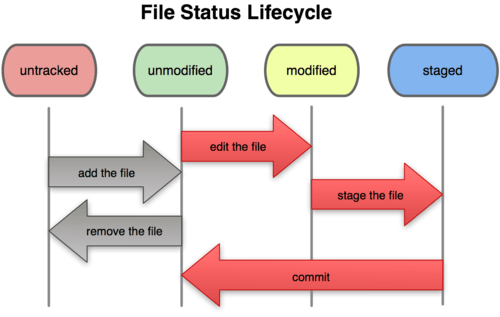
\includegraphics{2-1.png}
	\subsection{检查当前文件状态}
	要确定哪些文件当前处于什么状态,可以用\textbf{git status}命令。如果在克隆仓库之后立即执行此命令,会看到类似这样的输出:\\
	\fbox{
		\textbf{ \verb| $ vim README| \\}
		\textbf{ \verb| $ git status| \\}
		On branch master\\
		Untracked files:\\
		(use \verb| "git add <file>..." to include in what will be commited"|) \\

		\indent README

		nothing added to commit but untracked files present (use \verb| "git add" to track|)\\
	}
	在状态报告中可以看到新建的README文件出现在``Untracked files"下面。未跟踪的文件意味着Git在之前的快照(提交)中没有这些文件;Git不会自动将之纳入跟踪范围,除非你明明白白地告诉它``我们需要跟踪该文件",因而不用担心把临时文件什么的也归入版本管理。不过现在例子中,我们确实想要跟踪管理README这个文件。\\
	
	\subsection{跟踪新文件}
	\paragraph{}
	使用命令\textbf{git add}开始跟踪一个新文件。要跟踪README文件,运行:\\
	\fbox{
		\textbf{\verb|$ git add README|\\}
	}
	此时再运行\textbf{git status}命令,会看到README文件已被跟踪,并处于暂存状态。\\
	只要在``Changes to be commmitted"这行下面的,就说明是已暂存状态。如果此时提交,那么该文件此时此刻的版本将被留存在历史记录中。你可能 会想起之前我们使用\textbf{git init}后就运行了\textbf{git add}命令,开始跟踪当前目录下的文件,在\textbf{git add}后面可以指明要跟踪的文件或目录的话,就说明要递归跟踪该目录下的所有文件。(译注:其实\textbf{git add}的潜台词就是把目标文件快照放入暂存区域,也就是add file into staged area, 同时未曾跟踪过后文件标记为需要跟踪。这样就好理解后续的add 操作的实际意义了。)\\
	\subsection{暂存已修改文件}
	\paragraph{}
	现在我们修改下之前已跟踪过的文件然后:这里不想写了……,想看的话看原版吧。\\
	\subsection{忽略某些文件}
	\paragraph{}
	一般我们总会有些文件无需纳入Git的管理,也不希望它们总出现在未跟踪文件列表。通常都是些自动生成的文件,比如日志文件,或者编译过程中创建的临时文件等。我们可以创建一个名为\textbf{.gitignore}的文件,列出要忽略的文件模式。\
	如果你在里面写入\textbf{\verb| *.[oa] 或 *.~|}就是说以\textbf{.o}或\textbf{.a}结尾的文件和存档文件都是编译过程中出现的,我们用不着跟踪它们的版本。第二个波浪符是说副本文件也忽略。此外还有其他的不想说了。具体看规范如下:\\
	\begin{itemize}
		\item 所有窄或者以注释符号\verb|#|形状的行都会被Git忽略。
		\item 可以使用标准的glob模式匹配。
		\item 匹配模式最后跟反斜杠(/)说明要忽略的是目录。
		\item 要忽略指定模式以外的文件或目录,可以用模式前加上惊叹号(!)取反。
	\end{itemize}
	所谓的glob模式是指shell所使用的简化的正则表达式:
	\begin{itemize}
		\item 星号(*)匹配零或多个任意字符;
		\item \verb|[abc]|匹配任意一个或a或b或c;
		\item 问号只匹配一个任意字符;
		\item 在方括号中短划线分开两个字符如:\verb|[0-9]|或\verb|[a-f]|表示匹配它们中的所有字符。
	\end{itemize}
	\subsection{查看已暂存和未暂存的更新}
	\paragraph{}
	实际上\textbf{git status}的显示比较简单,仅仅是列出了修改过的文件,如果要查看具体修改了什么地方,可以用\textbf{git diff}命令。稍后我们会详细介绍。不过现在我们可以知道哪些更新哪些还暂存?哪些暂存了还没有提交?\textbf{git diff}会用文件补丁的格式显示具体添加和删除的行。\\
	\subsection{提交更新}
	\paragraph{}
	如果现在可以提交了,请在此之前,一定要确认还有什么修改过的或新建的文件还没有git add过,否则提交的时候不会记录这些没有暂存起来的变化。所以,每次准备提交前,先用\textbf{git status}看一下,是不是都已经暂存起来了,然后再运行提交命令\textbf{git commit}。\\
	\fbox{
		\textbf{\verb|$ git commit|\\}
	}
	这种方式会启动文本编辑器以便输入本次提交的说明。(默认会雇用shell的环境变量\verb|$EDITOR|所指定的软件,一般都是vim或emacs。\\
	在提交时也可以加上一个参数:\\
	\fbox{
		\textbf{\verb|$ git commit -m “I can play games with you"|\\}
	}
	好,现在已经创建了第一个提交!可以看到,提交后它会告诉你,当前是在哪个分支提交的,本次提交的完整SHA-1校验和(463d……),以及在本次提交中,有多少文件修订过,多少行添改和删改过。还有,每一次提交都是作一次快照,以后都可以回到这个状态,或者进行比较。\\
	\subsection{跳过使用暂存区域}
	\paragraph{}
	尽管使用暂存区域的方式可以精心准备要提交的细节,但有时候这么做略显繁琐。Git提供一个跳过使用暂存区域的方式,只要在提交的时候,用\textbf{git commit -a}就会自动把所有已经跟踪过的文件暂存起来一并提交,从而跳过\textbf{git add}步骤。\\
	\subsection{移除文件}
	\paragraph{}
	要从Git中移除某个文件,就必须要从已跟踪文件清单中移除(确切地说,是从暂存区域移除),然后提交。可以用\textbf{git rm}命令完成此项工作,并连带从工作目录中删除指定的文件,这样以后就不会出现在未跟踪文件清单中了。\\
	如果简单地从工作目录中手工删除文件,运行\textbf{git status}时就会在``Changes not staged for commit"部分(也就是\textit{未暂存}清单)看到。\\
	在删除文件或者目录的名字时也可以使用glob模式。不过星号之前要加反斜杠,因为Git有它自己的文件模式扩展匹配方式,所以我们不用shell来帮忙展开(译注:实际上不加反斜杠也可以运行,只不过按照shell扩展的话,仅仅删除指定目录下的文件而不会递归匹配。)\\
	\subsection{移动文件}
	\paragraph{}
	不像其他的VCS系统,Git并不跟踪文件移动操作。如果在Git中重命名了某个文件,仓库中存储的元数据不会体现出这是一次改名操作。不过Git非常聪明,它会推断出究竟发生了什么,至于具体是如何做到的,我们稍后再谈。\\
	既然如此,当你看到Git的mv命令时一定会困惑。要在Git中对文件改名,可以这样:\\
	\fbox{
		\textbf{ \verb| $ git mv file_from file_to|\\}
	}
	它会正常工作的。 实际上即使此时查看状态信息,也会明白地看到重命名的说明。\\
	我才不写呢,想看自己去试。\\

	\section{查看提交历史}
	\section{撤消操作}
	\section{远程仓库的使用}
	\section{打标签}
	\section{技巧和窍门}
	\section{小结}

\chapter{Git分支}

	\section{何谓分支}
	\section{分支的新建与合并}
	\section{分支的管理}
	\section{利用分支进行开发的工作流程}
	\section{远程分支}
	\section{分支的衍合}
	\section{小结}

\chapter{服务器上的Git}
	\section{协议}
	\section{在服务器上部署Git}
	\section{生成SSH公钥}
	\section{架设服务器}
	\section{公共访问}
	\section{GitWeb}
	\section{Gitosis}
	\section{Gitolite}
	\section{Git守护进程}
	\section{Git托管服务}
	\section{小结}

\chapter{分布式Git}
	\section{分布式工作流程}
	\section{为项目作贡献}
	\section{项目的管理}
	\section{小结}

\chapter{Git工具}
	\section{修订版本(Revision)选择}
	\section{交互式暂存}
	\section{储藏(Stashing)}
	\section{重写历史}
	\section{使用Git调试}
	\section{子模块}
	\section{子树合并}
	\section{总结}

\chapter{自定义Git}
	\section{配置Git}
	\section{Git属性}
	\section{Git挂钩}
	\section{Git强制策略实例}
	\section{总结}

\chapter{Git与其他系统}
	\section{Git与Subversion}
	\section{迁移到Git}
	\section{总结}
	
\chapter{git内部原理}
	\section{底层命令(Plumbing)和高层命令(Procelain)}
	\section{Git对象}
	\section{Git Refernces}
	\section{Packfiles}
	\section{The Refspec}
	\section{传输协议}
	\section{维护及数据恢复}
	\section{总结}



\end{document}
